\documentclass[11pt,letterpaper]{article}
\usepackage[T1]{fontenc}
\usepackage[utf8]{inputenc}
\usepackage{lmodern,microtype}
\usepackage[margin=0.94in,top=0.86in,bottom=0.86in]{geometry}
\usepackage{amsmath,amssymb,amsthm,mathtools}
\usepackage{booktabs,array,tabularx}
\usepackage{listings}
\usepackage{tikz}
\usetikzlibrary{arrows.meta,positioning,calc}
\usepackage{caption,float,graphicx,needspace}
\usepackage[hidelinks]{hyperref}
\hypersetup{pdfauthor={Thor Thor},pdftitle={RIFT: Reach-Invariant Firewall for Trust - Executable Static Reference Kernel},pdfsubject={Code-first security research manuscript},pdfkeywords={information flow,reachability,reference monitor,security invariant,RIFT}}
\urlstyle{same}
\setlength{\parindent}{1.25em}
\setlength{\parskip}{0pt}
\setlength{\abovecaptionskip}{5pt}
\setlength{\belowcaptionskip}{3pt}
\captionsetup{font=small,labelfont=bf}
\newtheorem{proposition}{Proposition}
\newtheorem{definition}{Definition}
\lstdefinestyle{rift}{language=Python,basicstyle=\ttfamily\footnotesize,columns=fullflexible,keepspaces=true,showstringspaces=false,frame=single,framerule=0.35pt,framesep=5pt,rulecolor=\color{black},breaklines=true,breakatwhitespace=true,aboveskip=7pt,belowskip=6pt}
\lstset{style=rift}
\renewcommand{\arraystretch}{1.11}
\begin{document}
\begin{center}
{\LARGE\bfseries RIFT: Reach-Invariant Firewall for Trust\par}
\vspace{5pt}
{\large An Executable Static Kernel for Pre-Commit Information-Flow Certification\par}
\vspace{14pt}
{\normalsize Thor Thor\par}
\vspace{3pt}
{\small Independent Open-Source Researcher, THOR-SEC\par}
{\small ORCID: \href{https://orcid.org/0009-0001-6573-385X}{0009-0001-6573-385X}\quad \texttt{codethor@gmail.com}\par}
{\small Repository: \url{https://github.com/codethor0/rift}\par}
{\footnotesize Independent research conducted on the author's own time; not sponsored by or representative of an employer.\par}
\vspace{5pt}
{\small Research paper, November 2026. Open for technical challenge.\par}
\end{center}
% Monochrome scientific illustration, kept with the title and above the abstract.
\begin{center}
\vspace{3pt}

\includegraphics[width=0.88\textwidth]{RIFT_Sphere_Flow_Figure.png}
\vspace{-10pt}
\end{center}
\vspace{3pt}
\begin{abstract}
\noindent RIFT provides an executable Python kernel for pre-commit certification over a \emph{finite, trusted, static} information-flow graph. For a supported mutation, it constructs a candidate state and decides \texttt{ALLOW}, \texttt{DENY}, or \texttt{UNKNOWN} using reachability from actual protected holdings to forbidden sinks. A counterexample found during adversarial review showed that topology deletion can erase evidence of a possible earlier transfer. The hardened kernel contains this defect by refusing \emph{every edge removal}: secure revocation and persistent taint are not implemented. The artifact includes source code, shortest-path witnesses, 37 regression tests, and an independent bounded DFS test oracle. These are model-relative results, not machine-checked verification or production enforcement.
\end{abstract}
\noindent\textbf{Keywords:} information flow; graph reachability; reference monitor; pre-commit certification; reproducible software; security invariants.
\clearpage
\section{Research artifact and scope}
The research objects are \path{src/rift_v3_static_candidate.py} and \path{tests/test_rift_v3_static_candidate.py}; Python 3.10+ and the standard library suffice. The graph describes \emph{physically possible} directed transfers, not permitted transfers. The finite-state predicate is meaningful only if a trusted environment supplies accurate holdings, labels, graph coverage, writer identities, and mediation of actual effects. The kernel does not establish these premises.
\begin{figure}[H]
\centering
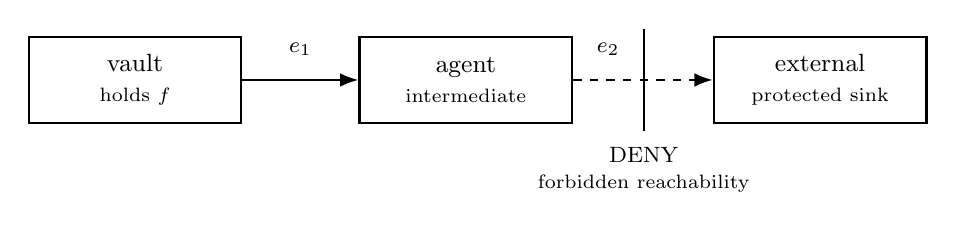
\begin{tikzpicture}[>=Latex,scale=1,every node/.style={transform shape},
    box/.style={draw,thick,minimum width=27mm,minimum height=11mm,align=center,font=\small}]
  \node[box] (vault) at (0,0) {vault\\\scriptsize holds $f$};
  \node[box] (agent) at (4.2,0) {agent\\\scriptsize intermediate};
  \node[box] (sink) at (8.7,0) {external\\\scriptsize protected sink};
  \draw[->,thick] (vault.east) -- node[above=5pt, font=\footnotesize] {$e_1$} (agent.west);
  \draw[->,thick,dashed] (agent.east) -- node[pos=.25,above=5pt,font=\footnotesize] {$e_2$} (sink.west);
  \draw[thick] (6.46,-0.65) -- (6.46,0.65);
  \node[anchor=north,font=\footnotesize,align=center] at (6.46,-0.73) {DENY\\\scriptsize forbidden reachability};
\end{tikzpicture}
\caption{The solid edge $e_1$ exists; dashed $e_2$ is proposed. The candidate would connect a held protected fact to a protected sink and is denied before local commit.}
\label{fig:reach}
\end{figure}

\subsection*{Trusted-boundary failure modes}
\begin{table}[H]
\centering\footnotesize
\begin{tabularx}{\linewidth}{@{}p{.23\linewidth}X@{}}\toprule
Trusted assumption & Failure mode when the assumption is false\\\midrule
Complete possible-flow graph & A missing edge can cause a false \texttt{ALLOW}; \texttt{coverage\_complete} is an externally supplied assertion, not coverage measurement.\\
Correct holdings and sensitivity & Missing holdings or misclassified facts can cause a false \texttt{ALLOW}; fact provenance is outside the kernel.\\
Authenticated writers and policy admins & A compromised identity may authorize unsupported policy intent; authentication and credential integrity are external.\\
Mediated physical transfers & A runtime transfer that bypasses certification is not represented by a committed graph transition and can violate real confidentiality.\\\bottomrule
\end{tabularx}
\caption{The guarantee is conditional on an explicitly trusted computing base; no enterprise coverage claim is made.}
\end{table}
\section{Formal model}
\begin{definition}[Finite state]
\begin{equation}\label{eq:model}\Sigma=(V,E,F,H,\lambda,P,g,c), \qquad P=(S,\tau,X,W,A,p_v).\end{equation}
Here $V$ is the node set, $E$ a directed multiset of stable-ID edges, $F$ the fact set, $H(u)\subseteq F$ the facts \emph{actually held} by node $u$, and $\lambda:F\to\{0,1,2\}$ the sensitivity label (public, internal, secret). $S\subseteq V$ is the protected-sink set, $\tau$ the minimum protected label, $X\subseteq F\times S$ explicit exceptions, and $W,A$ the writer and policy-administrator sets. The graph version is $g$, the policy version is $p_v$, and $c$ is a trusted coverage assertion.
\end{definition}
\noindent Let $u\leadsto_E s$ denote reflexive transitive reachability (including a zero-hop path). Then
\begin{equation}
B(\Sigma)=\{(u,f,s): f\in H(u),\; \lambda(f)\ge\tau,\; s\in S,\; u\leadsto_E s,\; (f,s)\notin X\}. \label{eq:bad}
\end{equation}
\noindent An action $a$ constructs a fully validated candidate $\Sigma'=T(\Sigma,a)$ without changing $\Sigma$. Two \emph{different} certification contracts are implemented:
\begin{align}
\operatorname{CLEAN}(\Sigma,a) &\iff B(\Sigma')=\varnothing, \label{eq:clean}\\
\operatorname{NO\_NEW}(\Sigma,a) &\iff B(\Sigma')\setminus B(\Sigma)=\varnothing. \label{eq:nonew}
\end{align}
\section{Decision procedure}
The in-process monitor requires a clean initial state and defaults to \texttt{CLEAN}; \texttt{NO\_NEW} is a weaker direct-certification option and must not be interpreted as remediation of existing violations.
\begin{table}[H]
\centering\small
\begin{tabularx}{\linewidth}{@{}lX@{}}\toprule
Result & Exact meaning in this implementation\\\midrule
\texttt{ALLOW} & Valid, authorized, supported candidate satisfies the selected finite-state predicate; monitor may commit locally.\\
\texttt{DENY} & Invalid input, unauthorized mutation, or a modeled forbidden path.\\
\texttt{UNKNOWN} & Incomplete coverage, stale version/nonce, unsupported change, or uncertified semantics. No commit.\\\bottomrule
\end{tabularx}
\caption{Three-valued certification. \texttt{UNKNOWN} is not an implicit permission.}
\end{table}
\noindent\textbf{Algorithm 1 (faithful abstraction of \texttt{certify} and \texttt{Monitor.submit}).}
\begin{lstlisting}[language={},basicstyle=\ttfamily\small]
Submit(Sigma, action, principal, contract=CLEAN):
  lock monitor; reject reused nonce as UNKNOWN
  validate state and action                  or DENY
  check writer and policy-admin authority    or DENY
  require complete coverage                  or UNKNOWN
  require current expected graph version     or UNKNOWN
  require increasing policy version          or DENY
  reject edge/holding/node removal, temporal or
    delegated semantics                      as UNKNOWN
  Sigma' := validated isolated candidate state
  old_bad := B(Sigma); new_bad := B(Sigma')
  failed := new_bad             if contract == CLEAN
         := new_bad - old_bad   if contract == NO_NEW
  reject unknown contract                    as UNKNOWN
  if failed is nonempty: return DENY + witnesses
  copy Sigma' into the monitor; record nonce
  return ALLOW
\end{lstlisting}
\noindent The actual source additionally validates exact built-in Python container types, node/fact/edge identities, exception references, authentication inputs, and policy versions. Local monitor commits are protected by a reentrant lock; this is \emph{not} a distributed transaction or a durable replay service.

\Needspace{37\baselineskip}
\section{Executable graph-search kernel}
The following is the core routine from the reference source, with its documentation string omitted for space. Breadth-first traversal records a parent map; witness paths are reconstructed only when a protected sink is reached.
\begin{lstlisting}[language=Python,basicstyle=\ttfamily\fontsize{8.4}{9.5}\selectfont]
def forbidden_flows(state: State) -> dict[tuple[str, str, str], Witness]:
    validate_state(state)
    edges = {n.id: [] for n in state.nodes}
    for edge in state.edges:
        edges[edge.src].append(edge.dst)
    facts = {f.id: f for f in state.facts}
    bad = {}
    for origin in state.nodes:
        for fid in origin.held_facts:
            if facts[fid].sensitivity < state.policy.min_protected:
                continue
            queue = deque([origin.id])
            parent: dict[str, Optional[str]] = {origin.id: None}
            while queue:
                current = queue.popleft()
                if (current in state.policy.protected_sinks and
                        (fid, current) not in state.policy.allowed_exceptions):
                    path = []
                    cursor: Optional[str] = current
                    while cursor is not None:
                        path.append(cursor)
                        cursor = parent[cursor]
                    w = Witness(origin.id, fid, current, tuple(reversed(path)))
                    bad[w.key] = w
                for nxt in edges[current]:
                    if nxt not in parent:
                        parent[nxt] = current
                        queue.append(nxt)
    return bad
\end{lstlisting}
\Needspace{4\baselineskip}
For each source/fact seed, graph exploration costs $O(|V|+|E|)$; reconstructed witnesses add output-dependent cost. This is an algorithmic bound for the finite in-memory graph, not a measured system latency or memory benchmark.

\section{Minimal reproducible example}
\begin{lstlisting}[language=Python]
from rift_v3_static_candidate import *
p = Policy(frozenset({'external'}))
s = State((Node('vault', frozenset({'f'})),
           Node('agent'), Node('external')),
          (), (Fact('f', Sensitivity.SECRET),), p)
m = Monitor(s)
print(m.submit(Action(0, 'a', add_edges=(
    Edge('read', 'vault', 'agent'),)), 'security-admin').decision.value)
print(m.submit(Action(1, 'b', add_edges=(
    Edge('send', 'agent', 'external'),)), 'security-admin').decision.value)
print(m.submit(Action(1, 'c', remove_edge_ids=('read',)),
               'security-admin').decision.value)
# ALLOW, DENY, UNKNOWN
\end{lstlisting}
\noindent Execute the bundled \path{examples/minimal_example.py} from the repository root with \texttt{PYTHONPATH=src python3 examples/minimal\_example.py}. The denied edge preserves the current committed version. The attempted edge removal is unsupported and also does not commit.

\section{Negative result: history cannot be erased by topology}
Adversarial review found a critical \emph{trace-level} failure in the earlier candidate: adding $\text{vault}\to\text{agent}$, removing that edge, and then adding $\text{agent}\to\text{external}$ could all be approved. While connected, the agent may have retained $f$; deleting topology cannot establish $f\notin H(\text{agent})$. This counterexample concerns successive committed states, not the shortest-path routine on an individual snapshot. The hardened release conservatively rejects the deletion.
\begin{table}[H]
\centering\small
\begin{tabularx}{\linewidth}{@{}cllX@{}}\toprule
Step & Proposed mutation & Hardened result & State consequence\\\midrule
1 & Add vault $\to$ agent & \texttt{ALLOW} & The read edge remains committed.\\
2 & Remove the read edge & \texttt{UNKNOWN} & No deletion; historical flow is not forgotten.\\
3 & Add agent $\to$ external & \texttt{DENY} & End-to-end forbidden path is detected.\\\bottomrule
\end{tabularx}
\caption{Conservative containment of historical-flow risk. This does not implement secure revocation.}
\end{table}
\noindent The safe containment is also a severe functional restriction: \emph{no edge can be removed through this monitor}. This is not delayed revocation; \emph{revocation is structurally unsupported}. A possible future design would maintain a monotone \texttt{may\_hold\_facts} set for each node, preserve it across edge removal, and separately certify privileged purge/declassification with evidence and auditability. That design is neither implemented nor validated here.

\section{Reproducibility and evidence}
\begin{table}[H]
\centering\small
\begin{tabularx}{\linewidth}{@{}l r X@{}}\toprule
Bundled evidence & Count & Interpretation\\\midrule
Python standard-library tests & 37 & Regression tests in \path{tests/test_rift_v3_static_candidate.py}.\\
Bounded static states & 512 & Enumerated small-state space in the bundled independent DFS test.\\
Single-edge proposals & 3,072 & Candidate certifications compared to an independent oracle.\\\bottomrule
\end{tabularx}
\caption{Reproducible, bounded evidence; not a universal proof of implementation or environment safety.}
\end{table}
\noindent\textbf{Execute:} \path{./run_tests.sh} from a clean checkout. The independent DFS oracle does not invoke the candidate's reachability routine. The earlier baseline had 27 tests; ten hardening regressions were added, yielding 37.
\par\medskip
\noindent\textbf{Reproducibility identifiers (SHA-256).}\par\smallskip
\noindent{\footnotesize\textbf{Signed hardened source commit:}\par}
\noindent{\footnotesize\ttfamily 763a41ff8588a545ee548b9c1562173cbc32aad5\par}
\smallskip\noindent{\footnotesize\textbf{Kernel source:} \path{src/rift_v3_static_candidate.py}\par}
\noindent{\footnotesize\ttfamily a3a83a1fb428f29d9c6795d083e1b81ec13bb85eb6ef13b925996f119fb6773a\par}
\smallskip\noindent{\footnotesize\textbf{Regression tests:} \path{tests/test_rift_v3_static_candidate.py}\par}
\noindent{\footnotesize\ttfamily e325e9abf1debc6cbef499eb1d522b99b794c57efbb8441dc3d3f708e3cb445f\par}
\smallskip
\noindent A later publication-only Git commit may differ; the final deposited ZIP manifest must identify its exact commit and include independent SHA-256 checksums of the PDF and software archive. These counts are bounded evidence, not a universal proof.
\par\medskip\noindent\textbf{Conditional invariant.} With a clean initial model and only \texttt{CLEAN}-certified local commits, every committed modeled state remains clean: the base case is clean, and each certified transition requires $B(\Sigma_{t+1})=\varnothing$. This elementary induction is a specification sanity check, \emph{not} a verified proof of the Python runtime or of real-world secrecy.

\section{Limits, operational refusals and future work}
\begin{table}[H]
\centering\footnotesize
\begin{tabularx}{\linewidth}{@{}p{.24\linewidth}X@{}}\toprule
Excluded mechanism & Why the present algorithm cannot certify it\\\midrule
Temporal paths and retained data & Snapshot BFS has no edge-lifetime semantics or durable may-have-held state; \emph{all} edge removals return \texttt{UNKNOWN}.\\
Delegation and declassification & Transferring authority or removing taint requires a stateful capability, provenance, and policy-administration model.\\
Distributed atomicity and crash recovery & A process-local lock and in-memory nonce set do not atomically mediate remote effects or survive process restart.\\
Covert/inference channels and unmediated effects & Graph reachability covers declared explicit paths only; information inferred or transferred outside mediation is invisible.\\
Production isolation and latency & No adversarial in-process isolation, operational p95/p99 measurements, or enterprise-scale topology study is supplied.\\\bottomrule
\end{tabularx}
\caption{Out-of-scope semantics and the missing mechanism that motivates each exclusion.}
\end{table}
\noindent\textbf{Cost of conservatism.} Valid operational edge deletion is refused even if no data actually moved; \texttt{UNKNOWN} is a noncommitting outcome, not a demonstrated leak. This limits applicability as a deployed monitor. Further, denial witnesses disclose fact IDs and complete modeled paths to authenticated writers, and rejected-input errors may echo supplied values. A multi-tenant deployment would need privileged diagnostic channels and output minimization; these protections are not implemented here.

\noindent\textbf{Research challenge.} Publish the exact source hash, initial \texttt{State} and \texttt{Policy}, action, principal, expected and actual decisions, and a minimal runnable reproducer. Distinguish a modeled false \texttt{ALLOW} from failure of external graph or mediation assumptions.

\section{Prior work and positioning}
The RIFT artifact does not claim to originate information-flow control or graph reachability. Denning's lattice model [1], Jif's security-typed Java [5], Flow Caml's information-flow type inference [6], and LIO's dynamic floating-label system [7] address related security properties at different enforcement boundaries.
\begin{table}[H]
\centering\footnotesize
\begin{tabularx}{\linewidth}{@{}p{.18\linewidth}p{.31\linewidth}X@{}}\toprule
Work & Principal technique & Boundary relative to RIFT\\\midrule
Denning [1] & Security classes and permitted flow relationships & Foundational lattice model, not this executable candidate-graph monitor.\\
Jif [5] & Static/dynamic checks in a security-typed Java language & Program information flows; RIFT checks proposed changes to a supplied finite graph.\\
Flow Caml [6] & Static security-type inference for OCaml & Language-level analysis rather than graph-mutation certification.\\
LIO [7] & Dynamic information-flow control with floating labels & Runtime label evolution; RIFT has no equivalent persistent label tracking.\\
RIFT (here) & Candidate-state graph reachability before local commit & Small auditable Python reference, with bounded tests and unsupported deletion.\\\bottomrule
\end{tabularx}
\caption{Qualitative positioning, not an empirical performance or superiority comparison.}
\end{table}
\noindent\textbf{Repository and release.} \url{https://github.com/codethor0/rift}. At public release, the software archive and checksum manifest must be deposited with this paper. The repository may remain private during manuscript review; its public accessibility must be checked before claiming an open release. Legacy research versions are not supported implementations.

\section*{References}
\small
\begin{enumerate}\setlength{\itemsep}{2pt}\setlength{\parskip}{0pt}
\item D. E. Denning, ``A Lattice Model of Secure Information Flow,'' \emph{Communications of the ACM}, vol. 19, no. 5, pp. 236--243, 1976.
\item A. Sabelfeld and A. C. Myers, ``Language-Based Information-Flow Security,'' \emph{IEEE Journal on Selected Areas in Communications}, vol. 21, no. 1, pp. 5--19, 2003.
\item T. Thor, ``Attack Calculus: A Typed, Evidence-Aware State-Transition Calculus for Cross-Domain Cybersecurity Reasoning,'' Zenodo, 2026. \url{https://doi.org/10.5281/zenodo.23092790}.
\item T. Thor, ``Memory-Egress Cryptographic Interlock: A Hardware-Enforced Capability-Separation Model for AI Memory Security,'' Zenodo, 2026. \url{https://doi.org/10.5281/zenodo.23109676}.
\item A. C. Myers, ``JFlow: Practical Mostly-Static Information Flow Control,'' \emph{Proceedings of the 26th ACM SIGPLAN-SIGACT Symposium on Principles of Programming Languages}, pp. 228--241, 1999.
\item F. Pottier and V. Simonet, ``Information Flow Inference for ML,'' \emph{ACM Transactions on Programming Languages and Systems}, vol. 25, no. 1, pp. 117--158, 2003. \url{https://doi.org/10.1145/596980.596983}.
\item D. Stefan, A. Russo, J. C. Mitchell, and D. Mazi\`eres, ``Flexible Dynamic Information Flow Control in Haskell,'' \emph{Proceedings of the ACM SIGPLAN Haskell Symposium}, pp. 95--106, 2011. \href{https://doi.org/10.1145/2034675.2034688}{doi:10.1145/2034675.2034688}.
\end{enumerate}
\normalsize
\end{document}
